
\chapter{Hierarchical mesh refinement with local time step}
\label{mesh_refinement}


Keeping the time step under a certain value relative to the element size in transitory problems is of key importance to achieve good results. Otherwise, an excessively large time step could resort on an over-diffusive solution.
Furthermore, the element size is governed by the physics, it has to be small enough to capture the modes of interest. It is a usual practice to refine the mesh near the region of interest or where the solution is changing rapidly. consequently, the local reduction of the mesh size is imposing a global reduction of the time step.

This section seeks for a strategy with emph{Local Time Step} (LTS). The main idea consists on the division on subdomains characterized by its mesh size. Thus, a hierarchic mesh refinement is defined with a characteristic mesh size and its corresponding time step. The hierarchical refinement allows to use both non-conforming discretization at space and at time level. The only requirement is having a natural number of divisions in order to perform a communication at the coarse level. Figure \ref{multilevel_refinement} shows a hierarchical spatial refinement.

This framework eases the refinement and coarsening procedures. Specially simple is the coarsening process, since it consists just on removing elements from a lower level without having to rebuild the connectivities. On the other hand, a procedure must be defined for the hanging nodes at the boundary and the hanging time steps.



\begin{figure}
    \centering
    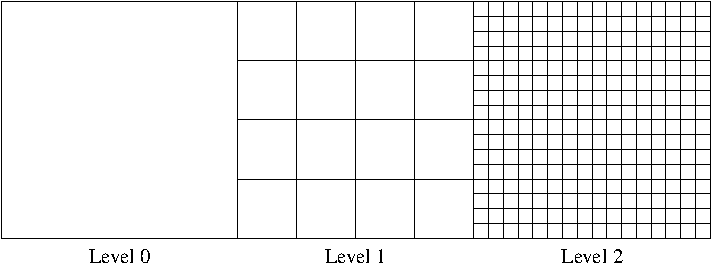
\includegraphics[width=.8\textwidth]{img/multigrid/multilevel_refinement.pdf}
    \caption{Two refinement levels. Each refinement has two levels of sub divisions.}
    \label{multilevel_refinement}
\end{figure}
% \begin{figure}
% \centering
% \begin{subfigure}{.8\textwidth}
%     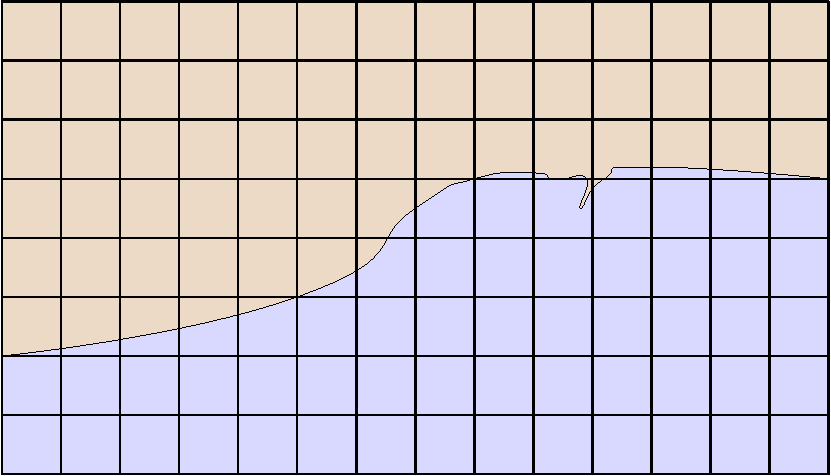
\includegraphics[width=\textwidth]{img/multigrid/grid1.pdf}
%     \vspace{1em}
% \end{subfigure}
% \begin{subfigure}{.8\textwidth}
%     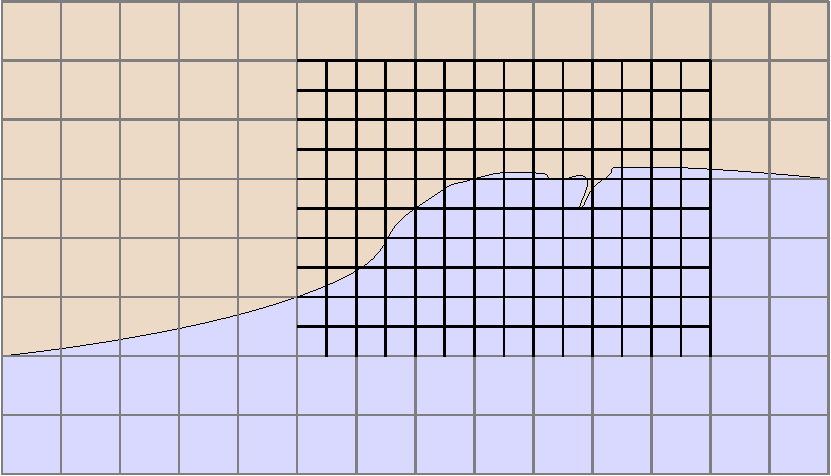
\includegraphics[width=\textwidth]{img/multigrid/grid2.pdf}
%     \vspace{1em}
% \end{subfigure}
% \begin{subfigure}{.8\textwidth}
%     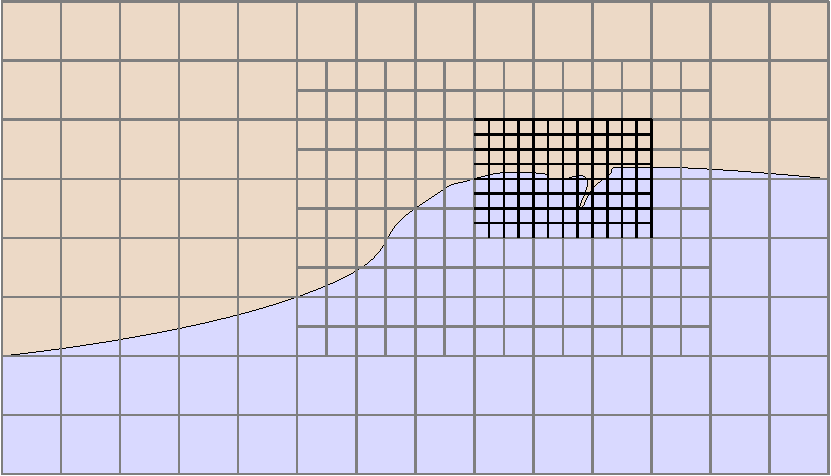
\includegraphics[width=\textwidth]{img/multigrid/grid3.pdf}
%     \vspace{1em}
% \end{subfigure}
% \caption{Different refinement zones for a domain.}
% \label{multigrid_refinement}
% \end{figure}


There have been previous advances in LTS. An early proposal can be found in \cite{chevalier1997}, where a LTS was proposed for waves propagation using the Maxwell's equations. The main interest of the LTS is the reduction of computational resources and to avoid the numerical diffusion caused by small time steps on coarse regions of the mesh. The cost of introducing a LTS with local mesh refinement i an instability at the coarse-fine interface. Collino analyzed the LTS for the hyperbolic 1D equations in \cite{collino2003a,collino2003b} and overcame this instability analyzing the conservation of discrete energy through refinement levels. Usually the LTS has been linked to explicit time steps.

DG have been successfully applied to overcome the stability constraint of explicit LTS. For example, in \cite{diaz2009} the non-conforming properties of DG are exploited to ensure stability. In that case, the continuity is enforced by the so-called numerical fluxes arising from the non conforming discretization of DG. On the other hand, CG is still a good solution, in \cite{almquist2016} stability is ensured by the classical technique of overlapping one coarse element with the fine mesh. A similar example can be found in \cite{grote2021}.

Finally, the most recent studies move towards massively parallel implementation. In \cite{baiges2016} a new library is presented. In this appendix, the implementation is designed in parallel processing, but without memory parallelization. On the other hand, attention is devoted to the algorithm, which is fully decoupled from the time integration, allowing for implicit or explicit schemes. In the future, this procedure can be easily extended to shared memory parallelization.


\section{Algorithm}

As stated in \cite{almquist2016,collino2003a}, the time step is driven by the finest mesh and the stability condition arising from the coarse-fine interface is overcome with a partial overlap. In the present case, the choice is to have a hierarchical structure of refined meshes fully overlapped, see Figure \ref{multilevel_overlap}. Apart from the advantages in parallel implementation, it allows to fully decouple the LTS from the time integration.

Having several meshes overlapped has an extra cost, since the coarse mesh has to be computed with the coarse time step at the refined region. However, its computational cost is insignificant in comparison with the resolution of the fine level. This step is considered as a predictor and is necessary for applying the boundary conditions at the fine level.

Hence, the stability relies on the boundary conditions applied to the fine level. The boundary conditions stated in chapter \ref{equations} does not necessary link all the variables, thus, some of the unknowns might not be continuous across the coarse-fine interface. This is the cost to pay for stability.

\begin{figure} [htpb]
    \centering
    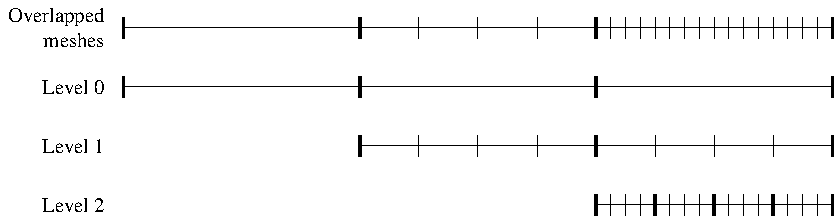
\includegraphics[width=\textwidth]{img/multigrid/multilevel_overlap.pdf}
    \caption{Unfolding of the overlapped hierarchical refinement for a 1D mesh.}
    \label{multilevel_overlap}
\end{figure}

Once defined the spatial refinement, the hanging nodes are included in the algebraic system using \emph{Multi-Point Constraints} (MPC). The values of a hanging node are computed by an average from the father nodes. This operation is performed recursively at all the divisions within the same hierarchic level.

Finally, after the prediction step of a coarse level, its sub-level is advanced with a smaller sub-step. Then, the interface is updated with the values from the prediction and is preceded to compute the solution of the sub-level. This procedure can be executed recursively. Once all the sub-steps have reached the step, the coarse predicted solution is updated with the values from the fine level. These steps are resumed in Figure \ref{multilevel_steps}.

\begin{figure} [htpb]
    \centering
    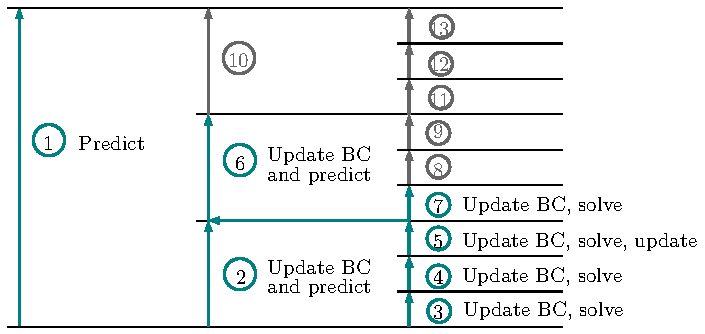
\includegraphics[width=.8\textwidth]{img/multigrid/multilevel_steps.pdf}
    \caption{Steps for solving a coarse time step with hierarchical refinement.}
    \label{multilevel_steps}
\end{figure}

It is important to remark that this procedure does not impose any restriction on having a discontinuity of refinement level higher than one. Regardless the jump of refinement level, the presented procedure is applied as well.



\section{Data structure}

The hierarchical refinement has been designed in order to be compatible with structured and unstructured meshes. Hence, the data structure is based on a finite element mesh, where nodes are defined by its coordinates and elements are defined by its connectivities.

The refinement begins when some elements are selected to refine according to a criterion which is to be defined. Then, those elements are copied to another mesh container identified by a consecutive refinement level. The nodes are also copied. It is important to remark that the copied nodes are only an auxiliary tool to define the connectivities. The mesh container identified with the refined level might contain elements already refined (Figure \ref{multilevel_meshing_steps}{\color{wrmBlue}a}). During the copying process, the destination nodes save a pointer to the origin node and vice-versa.

Once the coarse connectivities are transferred to the refined mesh, an iterative process begins to refine the elements and conditions until the desired refinement is achieved (Figure \ref{multilevel_meshing_steps}{\color{wrmBlue}b}). Every entity is split by inserting by dividing the edges into two. In the case of quadrilaterals, a node is added in the middle of the face, in the case of hexahedra, an extra node is added in the center of the volume. This operation requires some extra attention, because the edges and faces are shared by two elements. For this purpose, an auxiliary variable is defined in order to register the created entities. This variable is a map where the keys are the connectivities of the edge and the mapped value is the middle node. Each element has another variable storing the number of divisions performed, after executing a division, this value is incremented by one. This process is repeated until a specified number of divisions are reached.

\begin{figure}
    \centering
    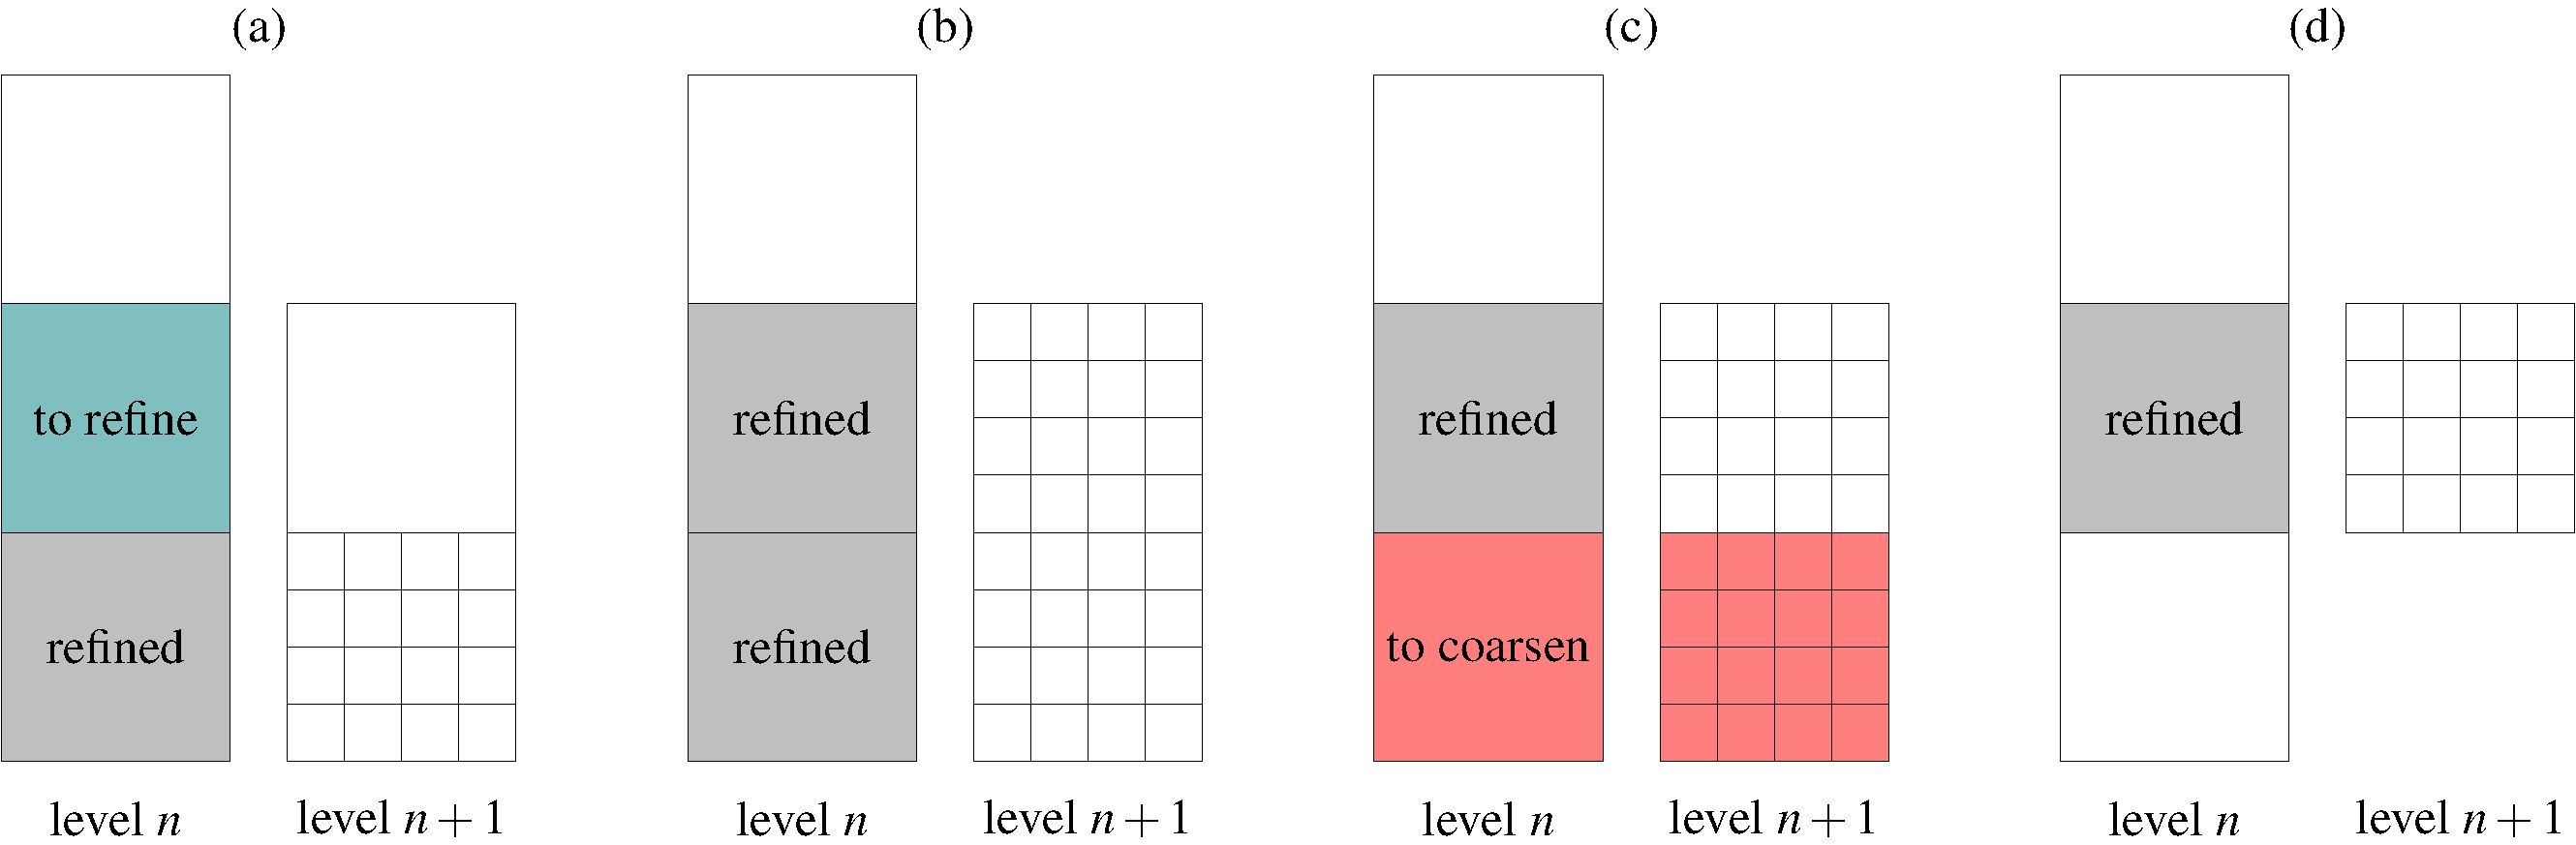
\includegraphics[width=\textwidth]{img/multigrid/multilevel_meshing_steps.pdf}
    \caption{Main steps for the refinement and coarsening process.}
    \label{multilevel_meshing_steps}
\end{figure}

The coarsening process is straightforward. It begins when the refinement criterion marks some elements at the coarse level to coarsen. This information is transferred to the refined elements using an auxiliary variable that allows to map from a refined element to its parent element. Hence, each refined element asks to the parent element if it is to be coarsened (Figure \ref{multilevel_meshing_steps}{\color{wrmBlue}c}).

The coarsening process is done by erasing all the elements to be coarsened from the refined level (Figure \ref{multilevel_meshing_steps}{\color{wrmBlue}d}). The process is finished by cleaning the hanging nodes and the auxiliary variables.
To sum up, the following variables are used by the refinement procedure:
\begin{description}
    \item[LEVEL] Scope: Mesh. The current refinement level.
    \item[REFINED] Scope: Elements, conditions. Flag indicating if the current entity has a nested refinement.
    \item[TO\_REFINE] Scope: Elements, conditions. Flag indicating if it must be refined.
    \item[TO\_COARSEN] Scope: Elements, conditions. Flag indicating if it must be coarsened.
    \item[FATHER\_NODES] Scope: Nodes. If the node is overlapped with a coarse node, there is only one father node and it points to the coarse node. If the current node is refined, it points to the nodes in the refined mesh.
    \item[FATHER\_NODES\_WEIGHTS] Scope: Nodes. The averaging of the nodal values. Has the same size than FATHER\_NODES and the sum of the wights is 1.
    \item[SLAVE\_NODE] Scope: Nodes. It points to a cloned node in the refined mesh.
    \item[FATHER\_ELEMENT] Scope: Elements, conditions. It points to the father entity at he coarse mesh.
    \item[NUMBER\_OF\_DIVISIONS] Scope: Elements, conditions. It counts how many times the entity has been divided.
    \item[NUMBER\_OF\_DIVISIONS] Scope: Mesh. It signifies how many times the entities had to be divided.
    \item[NODES\_MAP] Scope: Mesh. A map pointing to a refined node from the fathers nodes.
\end{description}


This can be easily implemented in parallel with the standard reduction techniques, except the NODES\_MAP. Adding new items to a map in parallel requires some extra architecture to ensure the thread safety. An alternative would be to split this map and reduce its scope to the nodes. It has some extra operations to write, read and remove values, but is worth for its scalability.



\section{Refinement criterion}

Finally, the refinement criterion has to be defined. There are two main criteria, the dynamic and the static one. The dynamic depends on the solution after the prediction step. In this case, the residual of the equations is evaluated -it is just the local right hand side before assembling the system when a residual-based system is used- and compared against a fixed value. When the local residual is too high, the element must be refined if there it has not been already refined. Whenever the local residual is sufficiently small, the element must be coarsened when it has a nested refinement.

The static criterion does not depend on the solution and the mesh is not modified during the analysis. This criterion serves to enhance the quality of the solution in a region. It is important to note that, by its hierarchical definition,  this refinement cannot be used to have a better definition of the boundaries. This algorithm is specially suited for the dynamic criterion.


\section{Examples}



